\begin{problem}[h]
<<echo=FALSE>>=
x_1 = round(runif(1,1,5))
x_2 = round(runif(1,8,15))
F_1 = round(runif(1,1,5))
F_2 = round(runif(1,8,15))
possible_angles = c(25,36,45,53,60,66,72,78,84)
angle = sample(possible_angles, 1)
cos_angulo_arred_p3 = round(cos(angle*pi/180),1)
#Result
displacement = x_2-x_1
work = F_1*cos_angulo_arred_p3*displacement-F_2*displacement
result_fake1 = F_1-F_2
result_fake2 = F_2-F_1*cos_angulo_arred_p3
result_fake3 = F_1-F_2*cos_angulo_arred_p3
result_fake4 = F_2-F_1
@
{\bf Work.} One particle walks over the X axis, changing its position from $x_1$=\Sexpr{(x_1)}m to $x_2$=\Sexpr{(x_2)}m. Two constant forces act on the particle. These are $F_1$=\Sexpr{(F_1)}N, which form an angle of \Sexpr{(angle)}\textdegree from the horizontal, and $F_2$=\Sexpr{(F_2)}N. Calculate the total work due to these two forces for the particule to go from $x_1$ to $x_2$.
 \begin{center}
    \begin{minipage}{8cm}
  		\begin{center}
        \begin{answers}{2}
          \bChoices[random]
            \Ans1 \label{resp4.3} \Sexpr{(work)}J\eAns 
            \Ans0 \Sexpr{(result_fake1)}J\eAns 
            \Ans0 \Sexpr{(result_fake2)}J\eAns  
            \Ans0 \Sexpr{(result_fake3)}J\eAns
            \Ans0 \Sexpr{(result_fake4)}J\eAns 
            \eFreeze
            \Ans0 None of them\eAns
          \eChoices 
        \end{answers} 
  		\end{center}
    \end{minipage}
  	\begin{minipage}{5cm}
  		\begin{center}
  				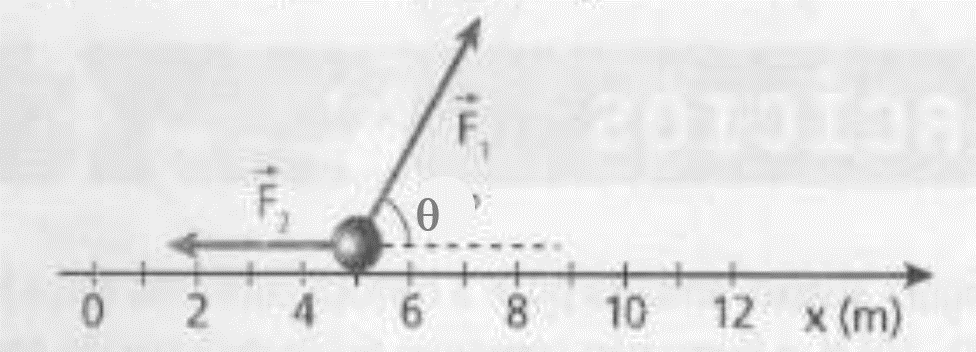
\includegraphics[width=6cm, height=3cm]{two_forces_question.png}
  		\end{center}
  	\end{minipage}
  \end{center}
\begin{solution}
Using the definition of Work, the total Work due to the two forces is:\\
$W=F_1\cdot d_{12}\cdot\cos\Sexpr{(angle)}^{\circ}+F_2\cdot d_{12}\cdot\cos 180^{\circ}=\Sexpr{(F_1)}N\cdot\Sexpr{(displacement)}m\cdot\Sexpr{(cos_angulo_arred_p3)}-\Sexpr{(F_2)}N\cdot\Sexpr{(displacement)}m=\Sexpr{(trabalho)}J$
\newline 
Therefore, the correct answer is the letter \textbf{(\REF*{resp4.3})}.
\end{solution}
\end{problem}